\documentclass[11pt, oneside, a4paper]{article}
\usepackage[utf8]{inputenc} % кодировка
\usepackage[english, russian]{babel} % Русские и английские переносы
\usepackage{graphicx}          % для включения графических изображений
\usepackage{cite}              % для корректного оформления литературы
\usepackage{enumitem}
\usepackage{pavt}                                
\usepackage{subfig}                                
\usepackage{multirow}                                
\renewcommand{\thesubfigure}{\asbuk{subfigure}}

% \usepackage{algorithmicx}
% \usepackage[ruled]{algorithm}
% \usepackage{algpseudocode}
% \usepackage[unicode=true,colorlinks,urlcolor=black,citecolor=black]{hyperref}
% \usepackage[unicode=true]{hyperref}
\usepackage{xcolor}
%\usepackage[]{hyperref}

\usepackage{url}

% correct bad hyphenation here
%\hyphenation{op-tical net-works semi-conduc-tor}

% Miscallaneous packages
\usepackage{color}

%\usepackage{fourier}

\newcommand\todo[1]{\textcolor{red}{\tiny ToDo: #1}}
%\newcommand\todo[1]{\textcolor{red}{\danger #1}}
\newcommand\note[1]{\textcolor{green}{\tiny Note: #1}}

\usepackage{listings}

%\usepackage{fancyhdr}
%\pagestyle{fancy}
%\lhead{}
%\chead{}
%\rhead{DRAFT 0.1}
%\renewcommand{\headrulewidth}{0.4pt}
%\renewcommand{\footrulewidth}{0.4pt}


\begin{document}
%
\title{Повышение эффективности параллельного языка программирования Charm++ для решения прикладных задач с мелкозернистым параллелизмом}


\authors{А.С.~Фролов\superscript{1}}
%\authors{А.С.~Фролов\superscript{1}, А.С.~Семенов\superscript{1}}
\organizations{АО "Научно-исследовательский центр электронной вычислительной техники"\superscript{1}}

\begin{abstract}

В статье рассматривается расширение программной модели Charm++ для повышения эффективности решения задач с 
мелкозернистым параллелизмом. Предлагаемое расширение заключается в поддержке специальных объектов – \textit{микро-chare} 
или (\textit{uchare-объектов}), наряду со стандартными Charm++ объектами (\textit{chare-объекты}), которые позволяют осуществлять 
декомпозицию задач на множество микро-chare объектов, количество которых может составлять десятки или сотни тысяч объектов на 
одно процессорное ядро. Такая мелкая гранулярность характерна для графовых алгоритмов, реализованных в парадигме 
\textit{vertex-centric}. Разработанный подход сравнивается с существующей методологией программирования параллельных задач на Charm++ 
на примере синтетического теста HPCC RandomAccess и одной из базовых графовых задач -- поиск вширь (breadth-first search),
более точно -- ее асинхронной версией (asynchronous breadth-first search). Дается оценка применения данного расширения в контексте 
программной модели программирования для экзафлопсных суперкомпьютеров.

\end{abstract}

\keywords{параллельная обработка больших графов, модели вычислений, программные модели, Charm++, экзафлопс}


\section{Введение}

% Мелкозернистый параллелизм 
% Что дает мелкозернистый параллелизм 
Мелкозернистый параллелизм -- одна из основополагающих идей многих новых, перспективных программных моделей, таких 
как X10 \cite{Charles2005}, HPX \cite{Kaiser2014}, Charm++ \cite{Kale1993} и др.
Мелкозернистый параллелизм подразумевает декомпозицию прикладной задачи на множество параллельных процессов (или нитей),
каждый из которых может состоять из небольшого числа команд (например, порядка 100 инструкций). Использование таких
``легких'' потоков позволяет обеспечить высокую загруженность процессорных ядер за счет быстрого переключения 
и отсутствия ожидания завершения длительных операцией (например, передачи данных по коммуникационной сети).
Достаточно часто легкие потоки используются в моделях вычислений, основанных на принципах управления вычислениями
потоком данных (или \textit{data-flow}), в частности, в моделях использующих \textit{активные} сообщения (Charm++ \cite{Kale1993}, 
ActivePebbles \cite{Willcock:2011:APP:1995896.1995934, willcock-active-pebbles}, SWARM и др.). 

%Charm++ 
Charm++ -- модель параллельного программирования, основанная на асинхронной модели управления потоком сообщений, представляющая
альтернативу классическому подходу к параллельному программированию, основанному на SPMD-модели. В конкретных реализациях SPMD могут 
использоваться библиотеки передачи сообщений, такие как Shmem или MPI, для распараллеливания на вычислительные узлы и средства 
распараллеливания внутри вычислительного узла (OpenMP, PThreads и др.). 

%Краткое описание Charm++ в одном абзаце
Базовым объектом в Charm++ является ``chare'' (или \textit{chare-объект}), обладающий помимо всех свойств объектов в С++ (инкапсулированными данными, 
множеством публичных и приватных методов и т.п.) интерфейсом из специальных entry-методов, вызовы которых соответствуют передаче данных 
(т.е. сообщений) между chare-объектами.  Приложение в Charm++ состоит из множества chare-объектов, обменивающихся между собой данными 
посредством вызовов \textit{entry-методов}. Кроме того, вызов entry-метода порождает выполнение непосредственно самого метода на том узле, где 
находится chare-объект, entry-метод которого был вызван, то есть таким образом реализуется концепция управления потоком данных или 
активных сообщений. 

% Charm++ и графовые приложения
Программная модель Charm++ естественным образом подходит для создания параллельных графовых приложений, так как многие из
графовых алгоритмов могут быть выражены в модели \textit{vertex-centric} \cite{McCune:2015:TLV:2830539.2818185} (VC-модель) и достаточно 
просто реализованы на Charm++. Так, каждая
вершина графа может быть представлена в виде chare-объекта, состояние которой описывается данными, привязанными к chare-объекту, а
программа состоит из множества параллельных процессов, выполняющихся над данными вершины и порождающими активные сообщения 
(в модели Charm++ активные сообщения реализованы в виде вызовов entry-методов).

% Свойства модели Charm++
Избыточная декомпозиция прикладной задачи -- один из основных принципов вычислительной модели Charm++, подразумевает то, что
задача будет разбита на столько отдельных частей на сколько возможно, и каждой из них будет назначен соответствующий chare-объект.
В случае графовых задач, когда каждой вершине графа соответствует chare-объект, количество chare-объектов может достигать 
нескольких миллиардов для больших графов или, соответственно, десятки (сотни) тысяч chare-объектов на одно ядро микропроцессора (PE). Такое
количество параллельных объектов может вызвать резкий рост накладных расходов со стороны системы поддержки параллельного 
выполнения Charm++ программ (runtime-системы). 

% ...
С другой стороны, выраженные в VC-модели графовые алгоритмы содержат большое количество обменов короткими 
сообщениями (типичная длина одного сообщения составляет несколько 64-разрядных слов), что понижает эффективности передачи 
данных по коммуникационной 
сети, так как увеличивается доля накладных расходов на служебные данные (заголовки сообщений, контрольные суммы и др.)
Для уменьшения накладных расходов на одно слово полезных данных стандартной практикой является агрегация коротких сообщений.
В Charm++ для агрегации сообщений существует специальная библиотека TRAM \cite{tramICPP14}, позволяющая не только агрегировать
короткие сообщения, но и создавать ``виртуальную топологию'' объединения процессов (PE) и осуществлять маршрутизацию сообщений 
в рамках виртуальной топологии с перекомпоновкой аргегированных пакетов на промежуточных узлах. Однако TRAM никак не решает проблему с 
большим количеством chare-объектов, описанную выше. Оценка эффективности TRAM для графовых
приложений является одной из задач данного исследования.

% 
Для увеличения производительности графовых приложений, выраженных в VC-модели, автором статьи разработана
специальная библиотека \textit{uChareLib}, расширяющая программную модель Charm++ дополнительным уровнем параллельных 
объектов -- ``микро-chare'' (\textit{uchare}) объектами, позволяющими создать необходимое количество объектов практически без
потери производительности.

В следующем разделе рассмотрена библиотека агрегации коротких сообщений TRAM. В третьем разделе представлена разработанная библиотека
uChareLib. Четвертый раздел содержит результаты оценок производительности трех подходов к созданию параллельных графовых приложений:
первый подход основан на использовании нативной Charm++ модели, второй подход -- на использовании библиотеки TRAM, третий -- на uChareLib.
В заключении содержатся выводы относительно применения Charm++ для разработки графовых приложений с использованием VC-модели.

%\section{Модель vertex-centric и ее реализации}
%\todo{???}

\section{Библиотека агрегации коротких сообщений TRAM}

% кратко
Основная идея библиотеки TRAM (Topological Routing and Aggregation Module) состоит в агрегации коротких сообщений,
передаваемых между chare-объектами, и организации программной маршрутизации агрегированных сообщений внутри 
``виртуальной топологии'', узлами которой являются процессы runtime-системы Charm++ (PE-процессы).
\footnote{
	Далее по тексту будет использоваться термин PE-процесс, что можно понимать как процессорное ядро,
	так как количество PE-процессов, как правило, равно количеству используемых ядер.
}

% подробно про маршрутизацию
В настоящее время в TRAM поддерживаются только решетчатые виртуальные топологии произвольной размерности 
(другое название TRAM -- NDMeshStreamer), 
однако при необходимости могут быть поддержаны и любые другие топологии. Для этих целей определен
класс VirtualRouter, который является базовым для конкретных реализаций топологий.
%\note{Не факт, в NDMeshStreamer очень много ориентировано именно на тор.}

\begin{figure}[!t]
\centering
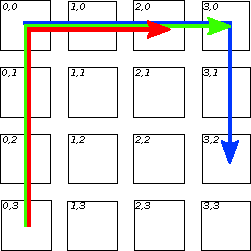
\includegraphics[width=0.4\linewidth]{img/tram_example.pdf}
\caption{Пример передачи сообщений в библиотеке TRAM}
\label{tram:example}
\end{figure}

% описание рисунка
На рисунке \ref{tram:example} показан пример агрегации коротких сообщений в виртуальной сети с топологией 2D-Mesh. Из рисунка видно, что 
посылаются следующие сообщения: $M_{(0,3)\rightarrow(2,0)}$, $M_{(0,3)\rightarrow(3,0)}$ и $M_{(0,0)\rightarrow(3,2)}$. При этом сообщения $M_{(0,3)\rightarrow(2,0)}$ 
и $M_{(0,3)\rightarrow(3,0)}$ пересылаются через промежуточный узел (0,0), что позволяет переслать их в одном агрегированном сообщении из узла (0,3) в узел (0,0).
Далее сообщения разделяются и $M_{(0,3)\rightarrow(2,0)}$ отправляется в узел назначения (2,0), а второе объединяется с сообщением $M_{(0,0)\rightarrow(3,2)}$
и пересылается в узел (3,0), который является узлом назначения для второго сообщения и промежуточным узлом для третьего. 
Таким образом, происходит объединение сообщений, маршруты которых имеют общие участки.   

% подробно про агрегацию
Данный подход к агрегации сообщений позволяет повысить эффективность агрегации (т.е. уменьшить общее количество передаваемых сообщений за счет повышения среднего
размера одного сообщения), сократить количество буферов необходимых для агрегации сообщений, более эффективно распределить трафик сообщений по коммуникационной 
сети.

\section{Библиотека микрообъектов uChareLib} 

% Концепция ucharelib
Библиотека uChareLib расширяет программную модель Charm++ новым типом объектов -- ``микро-chare'' (или uchare-объекты). Объекты данного типа 
наследуют все основные свойства стандартных chare-объектов, в том числе коммуникации посредством вызов entry-методов, коллективные операции
редукции и др. Единственным отличием uchare-объектов от chare-объектов заключается в том, что в отличие от chare-объектов вызовы entry-методов 
uchare-объектов планируются не в runtime-системе Charm++, а непосредственно в библиотеке uChareLib. Планировщик при этом максимально простой,
что позволяет сэкономить на переключении контекстов uchare-объектов, и, соответственно, создавать значительно большее количество uchare-объектов 
на один PE-процесс, чем это возможно с использованием стандартных chare-объектов.


\begin{figure}[!t]
\centering
\lstinputlisting[language=c++,
		basicstyle=\ttfamily\scriptsize\bfseries,
		morekeywords={mainchare, readonly, array, entry, reductiontarget, module, mainmodule, uchare, 1D}]
		{./img/hello.ci}
\caption{Пример Charm++ программы с массивом uchare-объектов (.сi файл)}
\label{ucharelib:example_ci}
\lstinputlisting[language=c++,
		basicstyle=\ttfamily\scriptsize\bfseries,
		morekeywords={mainchare, readonly, array, entry, reductiontarget, module, mainmodule, uchare, 1D}]
		{./img/hello.C}
\caption{Пример Charm++ программы с массивом uchare-объектов (.C файл)}
\label{ucharelib:example_C}
\end{figure}

% Описание примера
Для использования uchare-объектов необходимо добавить соответствующее объявление массива \textit{uchare array} в файл с расширением .ci, где
декларируются все объекты Charm++ программы и их entry-методы (см. рисунок \ref{ucharelib:example_ci}). По объявлениям, содержащимся в .ci-файле 
транслятором charmxi будут созданы файлы с расширениями .decl.h и .def.h, содержащие код с реализацией вспомогательных методов для создаваемых 
объектов, необходимых для отправки и приема сообщений, а также взаимодействия с runtime-системой Charm++. Данные файлы должны включаться в 
процесс компиляции Charm++ программы.

% Вызов entry-методов у uchare-объектов.
Обмен данными между uchare-объектами осуществляется аналогично обычным chare-объектам -- посредством вызовов entry-методов, определенных
в .ci файле. Вызов entry-методов uchare-объектов, также как и для обычных chare-объектов осуществляется через proxу-структуру, которая 
доступна через вызов getProxy (см. рисунок \ref{ucharelib:example_C}). 
Если entry-метод был вызван у uchare-объекта, находящегося в одном и том же PE-процессе вместе с объектом, инициировавшим
вызов, то вызов будет обработан немедленно, то есть так, как если бы это был вызов обычной функции или метода в С++ программе. В противном случае,
будет создано сообщение, содержащее идентификатор entry-метода, идентификатор uchare-объекта и аргументы вызова, которое будет доставлено в
PE-процесс, где находится заданный uchare-объект.

\begin{figure}[!t]
\centering
%\lstinputlisting{./img/hello.ci}
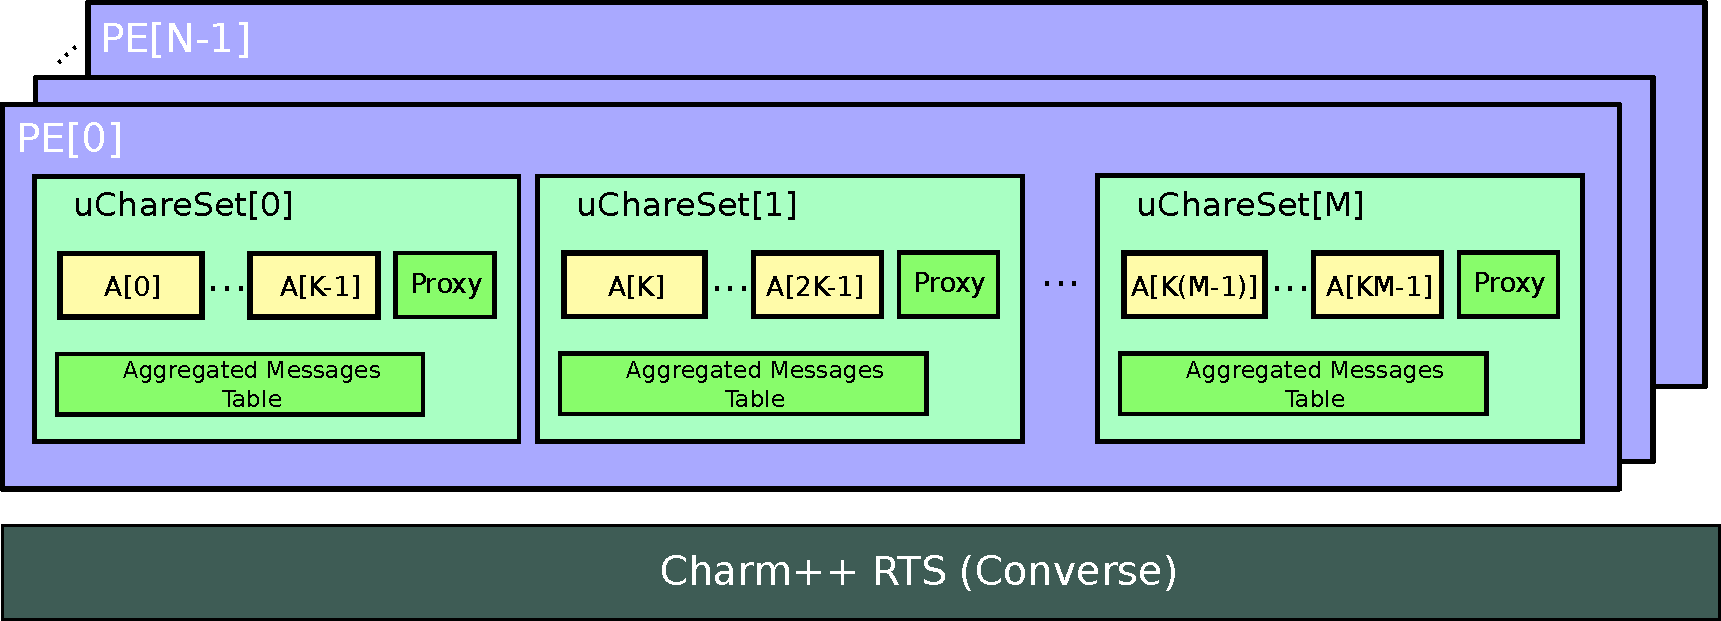
\includegraphics[width=0.7\linewidth]{img/ucharelib_overview.pdf}
\caption{Структура библиотеки uChareLib}
\label{ucharelib:overview} 
\end{figure}

% Детали реализации
Структура uChareLib приведена на рисунке \ref{ucharelib:overview}. В каждом PE-процессе создается несколько uChareSet объектов
(количество задается пользователем), между которыми равными частями делятся uchare-объекты (т.е. количество uchare-объектов должно
быть кратно количество uChareSet объектов). По сути uChareSet выполняет функцию менеджера uchare-объектов -- отвечает за отправку и
получение сообщений, планирует выполнения вызовов entry-методов.  

В uChareLib поддерживается два типа агрегации коротких сообщений. Первый -- наивная агрегация с использованием peer-to-peer (P2P)
агрегации, то есть для каждого uСhareSet создается таблица из $N-1$ буферов, где $N$ -- общее количество uChareSet объектов,
 которых происходит агрегация коротких сообщений, порождаемых при вызовах entry-методов uchare-объектов. Отправка агрегированного
сообщения происходит либо после переполнения буфера, либо принудительно с помощью вызова специальной функции flush. Второй способ 
подразумевает использование TRAM в качестве модуля для агрегации коротких сообщений. Стоит отметить, что для реализации данного
метода пришлось доработать программный интерфейс TRAM, так как в своем изначальном виде он оказался не совместим с uChareLib.
В результате получилась модифицированная версия TRAM -- TRAMx.

%The uChareLib source code as well as modified version of charmxi can be downloaded from \url{http://dislab.org/downloads/ucharelib}

\section{Оценка производительности}

\subsection{Набор оценочных тестов}

%\begin{itemize}
%\item RandomAccess, implementation of HPCC RandomAccess benchmark \cite{Luszczek:2006} on Charm++, TRAM, and uChareLib. The TRAM implementation 
%	 of RandomAcess from Charm++ source tree has been used.
%\item Asynchronous Breadth-First Search (BFS), algorithm for traversing graph vertices from the specified vertex (root). 
%   Asynchronous BFS differs from classic level-synchronous BFS used in Graph500 benchmark \cite{Graph500} in avoiding global synchronization
%	 after each level is passed. Therefore asynchronous BFS does not return parent tree with correct distances of the vertices from
%	 the root.
%\end{itemize}

% Описание тестов
Для оценки производительности были выбраны два оценочных теста: 
\begin{itemize}
\item Тест  HPCC RandomAccess\cite{Luszczek:2006}  реализует псевдослучайный доступ к большому массиву данных, единица измерения 
	производительности GUP/s (Giga Updates Per Second). 
\item Тест Asynchronous Breadth-First Search (ABFS) реализует поиск достижимых вершин в графе от заданной вершины (корня), 
	в отличие от стандартного BFS, используемого в Graph500 \cite{Graph500}, в асинхронном BFS отсутствует глобальная синхронизация после 
	обхода каждого уровня (т.е. решается задача только поиска достижимых вершин, без построения дерева предков). Единица измерения 
	производительности GTE/s (Giga Traversed Edges Per Second). 
\end{itemize}

Для каждого теста были сделаны три реализации: реализация на основе нативного Charm++, реализация на основе TRAM и
реализация на основе uChareLib. Кроме того, реализация на основе TRAM может использовать как оригинальную версию 
библиотеки, так и модифицированную (TRAMx). Также запуски тестов с использованием uChareLib осуществлялись с двумя
способами агрегации сообщений (P2P-агрегация и агрегация с использованием TRAM).

\subsection{Тестовые системы}

Использовались следующие вычислительные комплексы: 
\begin{itemize}
	\item вычислительный кластер МВС10П, установленный в МЦС РАН. МВС10П состоит из 1275 вычислительных узлов, каждый вычислительный узел
  имеет два 8-ядерных процессора Intel Xeon E5-2690 (2,9 Ггц) и 64 ГБ оперативной памяти. В качестве интерконнекта используется Infiniband FDR.
	\item 36-узловой тестовый кластер, установленный в АО <<НИЦЭВТ>> с коммуникационной сетью <<Ангара>> \cite{Angara1, Angara2}. Кластер 
	состоит из двух типов узлов: 24 двухпроцессорных узла с 6-ядерными процессорами Intel	Xeon E5-2630 (2,3 Ггц), 12 однопроцессорных узла с
	8-ядерными процессорами  Intel Xeon E5-2660	(2,2 Ггц). Все узлы имеют 64 ГБ оперативной памяти. Топология коммуникационной сети -- 3x3x4.
\end{itemize}

\subsection{RandomAccess}

\todo{дописать подробности реализации RandomAccess}

\begin{figure}[htb]
%\vspace{-1.5em}
\centering
\begin{tabular}{cccc}
\subfloat[МВС-10П]{\includegraphics[width=0.45\textwidth]{img/{plot.mvs10p.randomaccess.icc.n20.np64.ppn8}.pdf}} &
\subfloat[36-кластер с сетью <<Ангара>>]{\includegraphics[width=0.45\textwidth]{img/{plot.vertical.randomaccess.icc.n20.np64.ppn8}.pdf}} \\
\end{tabular}
\caption{Масштабируемость RandomAccess при увеличении количества chare-(uchare-) объектов на 
	один PE-процесс. Размер таблицы: $2^{20}$ записей на PE-процесс, количество узлов: 8, PE-процессов на узел: 8. 
	\todo{Обновить результаты для МВС-10П}
}
\label{benchmarking:randomaccess:chare-scalability}
%\vspace{-1.5em}
\end{figure}

% Описание рисунка
На рисунке \ref{benchmarking:randomaccess:chare-scalability} показана зависимость производительности
теста RandomAccess от количества используемых объектов. 
По графикам приведенным на рисунке можно сделать следующие выводы.
Во-первых, производительность нативной Charm++ реализации теста RandomAccess оказывается самой низкой,
при этом, при увеличении количества chare-объектов начаная с 1024, производительность Charm++ резко 
деградирует. 
Во-вторых, использование TRAM позволяет значительно (почти в 10 раз) повысить производительно RandomAccess,
однако при увеличении количества объектов также происходит стремительно падение производительности.
В-третьих, модифицированная версия TRAM (TRAMx) превосходит по производительности оригинальную версию
библиотеки, но также как Charm++ и TRAM подвержена падению производительности при большом количестве
chare-объектов.
В-четвертых, использование uchare-объектов (uChareLib) позволяет практически избежать падения производительности
даже при 64К uchare-объектах на один PE-процесс. Такой эффект говорит о том, что планирование uchare-объектов
внутри uChareLib осуществляется значительно более эффективно и создает меньшее количество накладных расходов.
Однако при малом числе объектов эффективность uChareLib оказывается ниже, чем TRAM и TRAMx 
(см. рис. \ref{benchmarking:randomaccess:chare-scalability}б). Такой результат 
возникает вследствие недостаточной эффективности механизма агрегации, использующегося в uChareLib и основанного
на P2P-подходе. Применение TRAM для агрегации сообщений внутри uChareLib позволило заметно повысить производительность,
но тем не менее производительность TRAM оказалась выше.

\begin{figure}[htb]
%\vspace{-1.5em}
\centering
\begin{tabular}{cccc}
\subfloat[МВС-10П, 1024 объекта/PE]{\includegraphics[width=0.45\textwidth]{img/{plot.mvs10p.randomaccess.icc.n20.chares1024.ppn8}.pdf}} &
\subfloat[36-кластер с сетью <<Ангара>>, 1024 объекта/PE]{\includegraphics[width=0.45\textwidth]{img/{plot.vertical.randomaccess.icc.n20.chares1024.ppn8}.pdf}} \\
\subfloat[МВС-10П, 16384 объекта/PE]{\includegraphics[width=0.45\textwidth]{img/{plot.mvs10p.randomaccess.icc.n20.chares16384.ppn8}.pdf}} &
\subfloat[36-кластер с сетью <<Ангара>>, 16384 объекта/PE]{\includegraphics[width=0.45\textwidth]{img/{plot.vertical.randomaccess.icc.n20.chares16384.ppn8}.pdf}} \\
\end{tabular}
\caption{Масштабируемость RandomAccess при увеличении количества вычислительных узлов. 
	Размер таблицы: $2^{20}$ записей на PE, количество chare-(uchare-) объектов: 1024 (a,б) 16384 (в,г) на PE, количество PE на узел -- 8}
\label{benchmarking:randomaccess:np-scalability}
\vspace{-2.0em}
\end{figure}

На рисунке \ref{benchmarking:randomaccess:np-scalability} показана зависимость производительности теста RandomAccess от количества
используемых узлов. Количество PE-процессов, запущенных на каждом узле -- 8 (т.е. использовалось 8 ядер), как для МВС-10П, так и для
кластера с сетью <<Ангара>>. Как видно из рисунка, для 1024 объектов на один PE-процесс, библиотека TRAM в целом показывает лучшую 
производительность, чем uChareLib (однако, на МВС-10П для 16 и 32 узлов uСhareLib обгоняет TRAM). 
Использование uChareLib совместно с TRAM позволяет увеличить производительность (см. рисунок \ref{benchmarking:randomaccess:np-scalability}б),
но не достаточно, для того чтобы сравняться с производительность TRAM.
При повышении количества объектов до 16384 на PE-процесс происходит изменение результатов и uChareLib значительно опережает TRAM,
что подтверждает предположение о том, что для задач с большим количеством объектов на один PE-процесс, использовать uchare-объекты
значительно эффективнее, чем стандартные chare-объекты.

%In addition to the RandomAccess implementation provided by the Charm++ developers as an example application of the TRAM library \cite{tramICPP14}, 
%another two implementations have been created. First uses native Charm++ programming model and almost identical to 
%the TRAM-based. Second uses the proposed uChareLib library.
%
%The updated table is evenly distributed between chares for native Charm++ and TRAM implementations and between uchares for uChareLib implementation
%of RandomAccess. Each chare (uchare) stores single contiguous block of the table of size equal to the ratio of the local table
%size to the number of chares (uchares). The global table size is increasing with number of PEs, that is the
%benchmark is a weak scaling problem. Each chare (uchare) generates a stream randomized updates to the global table
%which are created \todo{} by calls of the entry method \textit{update}.  
%
%Figure \ref{benchmarking:randomaccess:k1024} and Figure \ref{benchmarking:randomaccess:k16384} show scalability of the three different 
%implementations of the RandomAccess benchmark on MVS10P when the number of chares (or uchares when uChareLib is used) is 1K and 
%16K per each PE correspondingly. Variating the number of chares (uchares) per PE enable to control granularity of the 
%workload. 
%
%For the uChareLib four chares (uChareSets) per PE have been used and the performance results for two different values 
%(16 and 256) of aggregated message size are shown.
%
%As shown in Fig. \ref{benchmarking:randomaccess:k1024}, the native Charm++ implementation of the RandomAccess benchmark
%performs significantly slower than other implementations. The uChareLib implementation for small aggregated messages (maximum size is 16)
%shows improvement over pure Charm++ only on small number of nodes, which disappears when number of nodes is increased. 	The best 
%performance results, however, are shown by TRAM and uChareLib (when aggregated message size is 256) and for larger number of nodes
%uChareLib slightly outperforms TRAM.
%
%Performance results of RandomAccess for increased granularity of parallelism are shown in Fig. \ref{benchmarking:randomaccess:k16384}.
%First, it can be noted that the performance of the native Charm++ implementation has much not altered, while the performance of 
%the TRAM implementation has significantly decreased. At the same time performance of the uChareLib with increased aggregated message 
%size (256) is significantly better than TRAM for this case.
%
%Intermediate conclusion can be the following: the obtained results of the scalability of RandomAccess implemented on different 
%programming models showed that 
%while TRAM provide significant increase over pure Charm++ when moderate number of 
%chares are used per PE (less than 1K), it is not sufficiently effective comparing to uChareLib when number of chares per PE is
%extremely large.

%\subsection{Asynchronous Breadth-First Search}
\subsection{Асинхронный поиск вширь (Breadth-First Search)}

\begin{figure}[!t]
\centering
	\includegraphics[width=0.5\linewidth]{img/{plot.mvs10p.bfs.icc.n16.k16.ppn16}.pdf}
\caption{Производительность BFS на системе МВС-10П. Тип графа -- Erdos-Renyi 
	(RandomUniform graph with N= $2^{16}$, K=16 на PE-процесс, 16 PE-процессов на узел).
 \todo{добавить график для кластера с сетью <<Ангара>>}}
\label{benchmarking:bfs}
\end{figure}

%Breadth-First Search (BFS) is widely used graph analysis algorithm for searching all vertices of the graph which can be reached from 
%the specified vertex (or root). In canonical BFS algorithm the vertices are traversed in strict order of the level that is the distance
%from the root vertex. It requires performing barrier synchronization after each level is accomplished which is can be simply implemented 
%in classic message-passing (MPI) and/or shared memory (OpenMP) programming models. However, that is not effective way to implement BFS
%in Charm++ due to its asynchronous message-driven model. For the goals of this paper (comparing of different programming approaches
%to fine-grain parallel application)	it is sufficient to relax this requirement and compare results of \textit{asynchronous BFS}, that is
%BFS without intermidiate global synchronization.

Поиск достижимых вершин вширь (breadth-first search, BFS) очень часто используется в графовых задачах. В каноническом представлении
BFS обход вершин графа осуществляется в порядке их удаленности от корневой вершины, с которой начат поиск. Данное требование делает 
необходимым выполнение глобальной барьерной синхронизации после завершения обхода каждого ``уровня'' вершин, отстоящих от корневой вершины на
одинаковое расстояние. Выполнение барьерной синхронизации тривиально выражается в SPMD моделях параллельного программирования,
таких как MPI или OpenMP, однако такой подход не является оптимальный при реализации BFS на асинхронной модели с управлением потоком данных,
такой как Charm++. Для целей данной статьи (сравнение различных приемов программирования на Charm++ задач с ярко выраженным 
мелкозернистым параллелизмом) допустимым является пренебречь данным требованием и выполнить сравнение производительности асинхронного
варианта BFS -- ABFS, в котором отсутствует промежуточная глобальная барьерная синхронизация.

Для выполнения сравнения были разработаны три различные версии теста ABFS: нативная реализация на Charm++, реализация на базе TRAM
и реализация на основе uChareLib. Все три реализации сделаны в стиле vertex-centric, т.е. каждая вершина графа представлена или 
chare-объектом (нативная версия и версия на базе TRAM), или uchare-объектом (версия на базе uChareLib).

На рисунке \ref{benchmarking:bfs} приведены результаты запуска теста ABFS на вычислительном комплексе МВС-10П. На рисунке представлена 
зависимость производительности (GTE/s) от числа узлов. Количество используемых ядер – 16. Количество вершин графа N – 216, средняя 
степень связности вершин K – 16. Граф генерируется с равномерно случайным распределением дуг между вершинами (граф Erdos-Renyi).

Как видно из рисунка, производительность реализаций ABFS на Charm++ и TRAM одинакова. Использование uChareLib дает резкий прирост производительности 
в 40 раза. Также как и в случае с RandomAccess, производительность uChareLib крайне чувствительна к параметрам: Aggr.Max – максимальный размер 
агрегируемого сообщения и количеству chare-объектов (uСhareSet), используемых для агрегации uchare-объектов.

\section{Расширенная модель Charm++ для экзафлопсных суперкомпьютеров}


\begin{figure}[!t]
\centering
	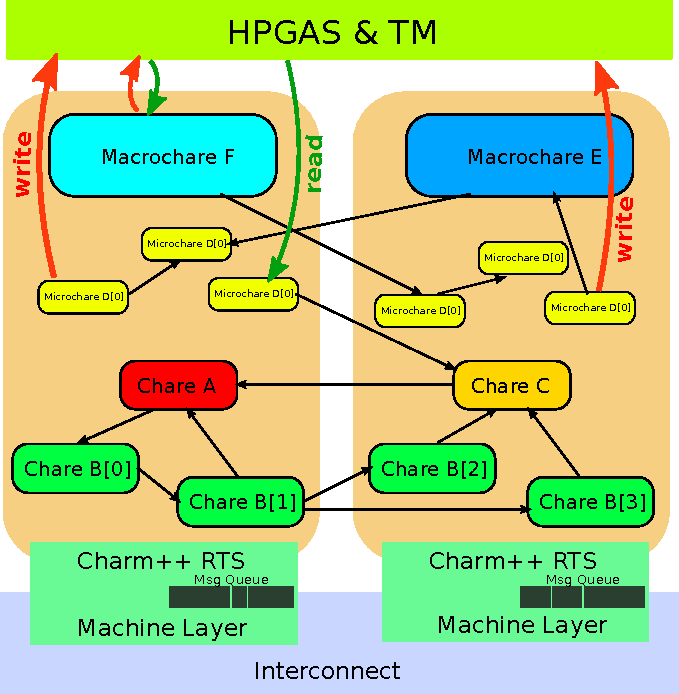
\includegraphics[width=0.5\linewidth]{img/charm-new-exec-model.pdf}
\caption{Расширенная программная модель Charm++}
\label{xcharm:model}
\end{figure}

Основные концепции модели Charm++ были разработаны почти 20 лет назад в то время, когда массово-параллельные системы (вычислительные кластеры) на основе коммерческих микропроцессоров только набирали популярность. Тем не менее, модель Charm++, вобравшая в себя как принципы dataflow-моделей, так и многопоточных (мультитредовых) моделей вычислений, оказалась достаточно успешной и с момента создания почти не претерпевала изменений. Однако, за этот период архитектура вычислительных систем существенна изменилась, а с появлением экзафлосных суперкомпьютеров разница архитектур станет еще значительней

Таким образом, сохранение основных принципов программной модели Charm++ (управление потоком сообщений, асинхронность, инкапсулированность данных), введение расширений, отражающих новые архитектурные возможности суперкомпьютеров, а также соответствие классу задач обработки больших графов – суть методологии создания новой программой модели, описываемой в данной статье. Схематически предлагаемая расширенная программная модель Charm++ приведена на рисунке \ref{xcharm:model}. 
Ниже приведены описания предлагаемых расширений к Charm++.

\textit{Классификация chare-объектов по целевой архитектуре.} Для соответствия гибридной архитектуре вычислительных узлов экзафлосных вычислительных систем, включающей в себя вычислительные ядра разного типа (CPU, GPU, FPGA), предлагается расширить тип chare-объекта Charm++ соответствующим спецификатором. Для реализации предлагается ввести соответствующие ключевые слова в язык интерфейса Charm++. Система поддержки выполнения Charm++ программ (runtime-система) будет автоматически распределять chare-объекты по соответствующим вычислительным ядрам узла суперкомпьютера. 

\textit{Классификация chare-объектов по гранулярности параллелизма.} Также предлагается разделять chare-объекты по степени гранулярности параллелизма (т.е. объему данных, содержащихся внутри объекта, и количеству команд процессора, требуемых для выполнения entry-методов). Предлагается ввести три типа объектов: микро, нормальный и макро. В соответствии с названиями микро-chare-объекты будут соответствовать самым малым вычислительным единицам параллельного алгоритма (таких объектов на одном ядре может выполняться до десятков тысяч), нормальные chare-объекты соответствуют обычным Charm++ объектам, макро-chare-объекты будут соответствовать наиболее "тяжелым" вычислениям, требующим большого количества данных, и включать entry-методы, состоящие из большого числа инструкций (например, содержать вложенные циклы и т.п.). Такая специализация позволит runtime-системе оптимизировать хранение chare-объектов и обеспечить наиболее эффективное планирование выполнения entry-методов. Для реализации предлагается ввести соответствующие ключевые слова в язык интерфейса Charm++. 

\textit{Динамические домены синхронизации.} Использование динамических доменов синхронизации позволит повысить эффективность и масштабируемость приложений, в которых предполагается выполнение какой-либо синхронизации (барьера, определения состояния завершения всех entry-методов и т.п.)  по динамически определяемому подмножеству chare-объектов. Данная операция требуется во многих графовых алгоритмах и их асинхронных реализациях (например, в алгоритме Борувки поиска минимального остовного дерева графа).

\textit{Многоуровневая глобально адресуемая распределенная общая память (HPGAS).} Изначально программная модель Charm++ не предполагает использования общей памяти как таковой. Все chare-объекты работают только с локальными данными, что позволяет перемещать chare-объекты между вычислительными узлами. Однако для некоторых алгоритмов введение общей памяти позволяет упростить реализацию и повысить эффективность. Предлагаемые уровни иерархии должны включать: уровень кэш-памяти (L1-L3 кэши), уровень сверхбыстрой памяти (HBM-памяти), уровень локальной памяти (DDR4), уровень локальной NVRAM, уровень удаленной памяти, доступной через RDMA операции. Данные должны размещаться в подсистеме памяти в соответствии с указанным уровнем, что позволит обеспечить максимальную гибкость в управлении доступом к памяти. 

\textit{Поддержка проблемно-ориентированных языков программирования.} Расширение возможностей программной модели Charm++ может привести к усложнению программирования. Данная проблема может быть решена за счет использования проблемно-ориентированных языков программирования (DSL). Для работы с графами может быть использован язык Green-Marl \cite{Hong:2012:GDE:2150976.2151013} или другие языки для работы с графами (в том числе языки запросов к графовым базам данных).
Представленный перечень расширения программной модели Charm++ не является окончательным, и его уточнения будет проводиться в ходе дальнейших исследований.

\section{Заключение}

%Fine-grained parallelism provides many numerous possibilities for exploiting hybrid many-core architectures of existing and future HPC systems. 
%However, high granularity of parallelism can cause performance problems as it incurs overheads from runtime system to schedule parallel
%threads to executions as well as modern interconnects do not effectively support short message communication which also cause 
%performance degradation and scalability problems of end-user applications. 
%
%Charm++ programming model stimulate users to use overdecomposition of their problems. However, when of number chares is more than 1K
%Charm++ runtime is overloaded and useful CPU utilization decreases significantly. The existing tools such as TRAM can mend this issue
%but in some cases (when number of chares is extreamly high) it is not sufficiently effective. 
%
%For such cases uChareLib library is proposed. It indroduces the concept of uchares which are incorporated into usual Charm++ chares
%and scheduled inside uChareLib. Performance evaluation on two benchmarks (RandomAccess and Asynchronous BFS) showed significant 
%improvement of uChareLib over Charm++ and TRAM.
%
%uChareLib is not restricted to graph applications only and can be used in different application areas where fine-grained parallelism 
%is achieved (such as molecular dynamics, adaptive irregular meshes, bioinformatics, etc.). Also uChareLib can be used with standard Charm++ 
%techniques in single application.
%
%For future research the next directions can be considered. First, enhancing uchare programming model with more possibilities such as
%using light-weight synchronization techniques, etc., or inserting specialization of uchares relative to extensively heterogeneous
%architecture of modern supercomputers. Second, it can be worthwhile to assess possibility of integrating uchares directly
%into Charm++ runtime system preserving that minimalistic shceduling and aggregation principles which implemented in uChareLib. Third,
%it is certainly needed to compare Charm++ with other programming models such as PBGL, Active Pebbles, Grappa focused on large-scale graph
%applications.

В статье представлена библиотека uChareLib для поддержки микрообъектов (uchare-объектов) в языке Charm++. Использование uchare-объектов
позволяет значительно повысить производительность программ на Charm++, в которых количество объектов на один процесс (или что практически 
то же самое одно ядро) составляет десятки тысяч. 	
 
Показан эффект от одного из предлагаемых расширений – поддержки микро-chare-объектов, на двух тестах HPCC RandomAccess и Asynchronous BFS. 
Ускорение, полученное от использования микро-chare-объектов, составило 5 раз для RandomAccess и 40 раза для ABFS на МВС-10П. Для 36-узлового 
кластера с сетью «Ангара» на тесте RandomAccess ускорение uChareLib относительно библиотеки TRAM составило 3 раза. Тем не менее, данные 
результаты являются предварительными и в будущем планируется провести оценочное тестирование с большим числом параметров исследуемых библиотек 
(uChareLib, TRAM) и оценочных тестов и на большем числе узлов. Дальнейшие планы по данному направлению включают исследование uСhareLib на разнообразных графовых 
задачах и большом числе узлов, реализацию остальных предложенных расширений модели Charm++.

На основании полученных результатов можно сделать вывод, что для задач, в которых количество chare-объектов достаточно большое (превышает 
1К на один PE-процесс), использование Charm++ и TRAM будет малоэффективно. Применение библиотеки uChareLib позволит 
значительно повысить эффективность задач с мелкозернистым параллелизмом.

%\textbf{Acknowledges\\}
%\section*{Acknowledgment} 
Данная работа выполнена при поддержке Российского Фонда Фундаментальных Исследований (грант №15-07-09368).

\bibliography{mypapers.bib}{}
%\bibliographystyle{plain}
\bibliographystyle{unsrt}

\onecolumn
\newpage

\end{document}


